\hypertarget{the-falikov-kimball-model}{%
\section{The Falikov Kimball Model}\label{the-falikov-kimball-model}}

\hypertarget{the-model}{%
\subsection{The Model}\label{the-model}}

The Falikov-Kimball (FK) model is one of the simplest models of the correlated electron problem. It captures the essence of the interaction between itinerant and localized electrons. It was originally introduced to explain the metal-insulator transition in f-electron systems but in its long history it has been interpreted variously as a model of electrons and ions, binary alloys or of crystal formation~\autocite{hubbardj.ElectronCorrelationsNarrow1963,falicovSimpleModelSemiconductorMetal1969,gruberFalicovKimballModelReview1996,gruberFalicovKimballModel2006}. In terms of immobile fermions \(d_i\) and light fermions \(c_i\) and with chemical potential fixed at half-filling, the model reads

\[\begin{aligned}
H_{\mathrm{FK}} = & \;U \sum_{i} (d^\dagger_{i}d_{i} - \tfrac{1}{2})\;(c^\dagger_{i}c_{i} - \tfrac{1}{2}) -\;t \sum_{\langle i,j\rangle} c^\dagger_{i}c_{j}.\\ 
\end{aligned}\]

Here we will only discuss the hypercubic lattices, i.e~the chain, the square lattice, the cubic lattice and so on. The connection to the Hubbard model is that we have relabel the up and down spin electron states and removed the hopping term for one species, the equivalent of taking the limit of infinite mass ratio~\autocite{devriesSimplifiedHubbardModel1993}.

Like other exactly solvable models~\autocite{smithDisorderFreeLocalization2017} and the Kitaev Model, the FK model possesses extensively many conserved degrees of freedom \([d^\dagger_{i}d_{i}, H] = 0\). The Hilbert space therefore breaks up into a set of sectors in which these operators take a definite value. Crucially, this reduces the interaction term \((d^\dagger_{i}d_{i} - \tfrac{1}{2})\;(c^\dagger_{i}c_{i} - \tfrac{1}{2})\) from being quartic in fermion operators to quadratic. This is what makes the FK model exactly solvable, in contrast to the Hubbard model.

Due to Pauli exclusion, maximum filling occurs when each lattice site is fully occupied, \(\langle n_c + n_d \rangle = 2\). Here we will focus on the half filled case \(\langle n_c + n_d \rangle = 1\). The ground state phenomenology as the model is doped away from the half-filled state can be rich~\autocite{jedrzejewskiFalicovKimballModels2001,gruberGroundStatesSpinless1990} but from this point we will only consider the half-filled point.

At half-filling and on bipartite lattices, FK the model is particle-hole (PH) symmetric. That is, the Hamiltonian anticommutes with the particle hole operator \(\mathcal{P}H\mathcal{P}^{-1} = -H\). As a consequence the energy spectrum is symmetric about \(E = 0\) and this is the Fermi energy. The particle hole operator corresponds to the substitution \(c^\dagger_i \rightarrow \epsilon_i c_i, d^\dagger_i \rightarrow d_i\) where \(\epsilon_i = +1\) for the A sublattice and \(-1\) for the even sublattice~\autocite{gruberFalicovKimballModel2005}. The absence of a hopping term for the heavy electrons means they do not need the factor of \(\epsilon_i\). See appendix \protect\hyperlink{particle-hole-symmetry}{A.1} for a full derivation of the PH symmetry.

\hypertarget{fig:simple_DOS}{%
\begin{figure}
\centering
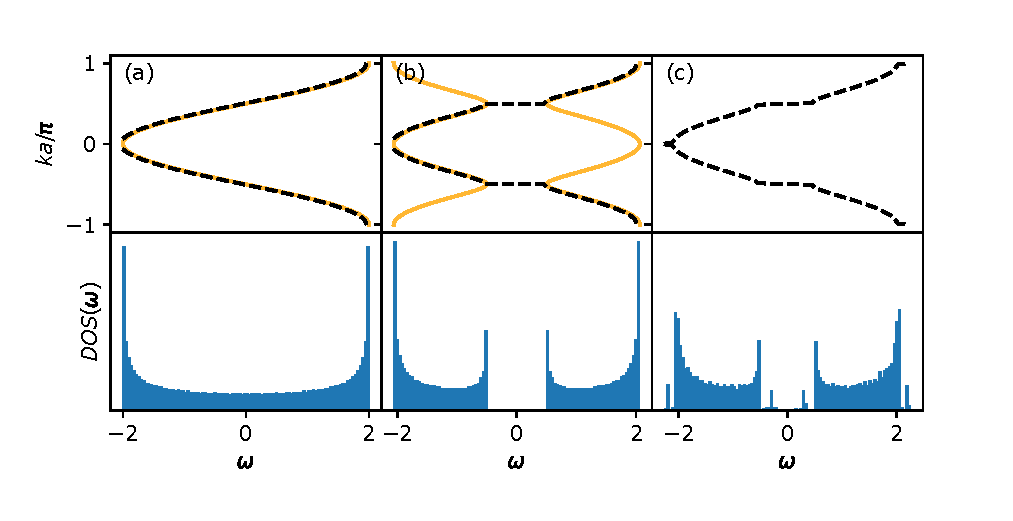
\includegraphics[width=1\textwidth,height=\textheight]{figure_code/background_chapter/simple_DOS}
\caption[{Cubic Lattice dispersion with disorder}]{The dispersion (upper row) and density of states (lower row) obtained from a cubic lattice model \(H = \sum_{i} V_i c^\dagger_{i}c_{i} - t \sum_{\langle i,j\rangle} c^\dagger_{i}c_{j}\) in one dimension. (a) With not external potential. (b) With a static charge density wave background \(V_i = (-1)^i\) (c) A static charge density wave background with 2\% binary disorder.}
\label{fig:simple_DOS}
\end{figure}
}

We will later add a long range interaction between the localised electrons at which point we will replace the immobile fermions with a classical Ising field \(S_i = 1 - 2d^\dagger_id_i = \pm\tfrac{1}{2}\) which I will refer to as the spins.

\[\begin{aligned}
H_{\mathrm{FK}} = & \;U \sum_{i} S_i\;(c^\dagger_{i}c_{i} - \tfrac{1}{2}) -\;t \sum_{\langle i,j\rangle} c^\dagger_{i}c_{j}.\\ 
\end{aligned}\]

The FK model can be solved exactly with dynamic mean field theory in the infinite dimensional~\autocite{antipovCriticalExponentsStrongly2014,ribicNonlocalCorrelationsSpectral2016,freericksExactDynamicalMeanfield2003,herrmannNonequilibriumDynamicalCluster2016}.

\hypertarget{phase-diagrams}{%
\subsection{Phase Diagrams}\label{phase-diagrams}}

\hypertarget{fig:fk_phase_diagram}{%
\begin{figure}
\centering
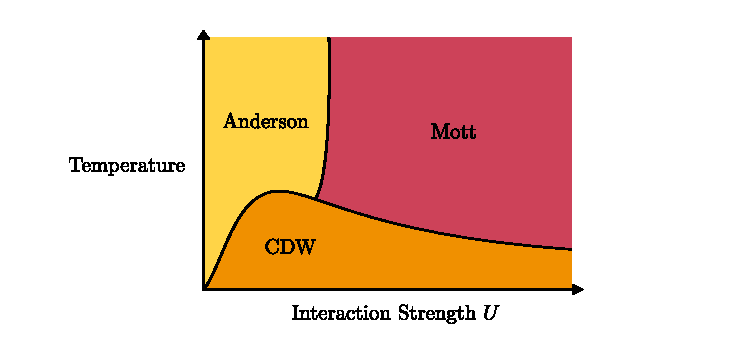
\includegraphics[width=1\textwidth,height=\textheight]{figure_code/background_chapter/fk_phase_diagram}
\caption[{Fermi-Hubbard and Falikov-Kimball Temperatue-Interaction Phase Diagrams}]{Schematic Phase diagram of the Falikov-Kimball model in dimensions greater than two. At low temperature the classical fermions (spins) settle into an ordered charge density wave state (antiferromagnetic state). The schematic diagram for the Hubbard model is the same. Reproduced from~\autocite{antipovInteractionTunedAndersonMott2016,antipovCriticalExponentsStrongly2014}}
\label{fig:fk_phase_diagram}
\end{figure}
}

In dimensions greater than one, the FK model exhibits a phase transition at some \(U\) dependent critical temperature \(T_c(U)\) to a low temperature ordered phase \autocite{maskaThermodynamicsTwodimensionalFalicovKimball2006}. In terms of the immobile electrons this corresponds to them occupying only one of the two sublattices A and B this is known as a charge density wave (CDW) phase. In terms of spins this is an AFM phase.

In the disordered region above \(T_c(U)\) there are two insulating phases. For weak interactions \(U << t\), thermal fluctuations in the spins act as an effective disorder potential for the fermions, causing them to localise and giving rise to an Anderson insulating state~\autocite{andersonAbsenceDiffusionCertain1958} which we will discuss more in section~\protect\hyperlink{bg-disorder-and-localisation}{2.3}. For strong interactions \(U >> t\), the spins are not ordered but nevertheless their interaction with the electrons opens a gap, leading a Mott insulator analogous to that of the Hubbard model~\autocite{brandtThermodynamicsCorrelationFunctions1989}.

By contrast, in the one dimensional FK model there is no finite-temperature phase transition (FTPT) to an ordered CDW phase~\autocite{liebAbsenceMottTransition1968}. Indeed dimensionality is crucial for the physics of both localisation and FTPTs. In one dimension, disorder generally dominates: even the weakest disorder exponentially localises \emph{all} single particle eigenstates. Only longer-range correlations of the disorder potential can potentially induce localisation-delocalisation transitions in one dimension~\autocite{aubryAnalyticityBreakingAnderson1980,dassarmaLocalizationMobilityEdges1990,dunlapAbsenceLocalizationRandomdimer1990}. Thermodynamically, short-range interactions cannot overcome thermal defects in one dimension which prevents ordered phases at non-zero temperature~\autocite{goldshteinPurePointSpectrum1977a,abrahamsScalingTheoryLocalization1979,kramerLocalizationTheoryExperiment1993}.

However, the absence of an FTPT in the short ranged FK chain is far from obvious because the Ruderman-Kittel-Kasuya-Yosida (RKKY) interaction mediated by the fermions~\autocite{kasuyaTheoryMetallicFerro1956,rudermanIndirectExchangeCoupling1954,vanvleckNoteInteractionsSpins1962,yosidaMagneticPropertiesCuMn1957} decays as \(r^{-1}\) in one dimension~\autocite{rusinCalculationRKKYRange2017}. This could in principle induce the necessary long-range interactions for the classical Ising background to order at low temperatures~\autocite{thoulessLongRangeOrderOneDimensional1969,peierlsIsingModelFerromagnetism1936}. However, Kennedy and Lieb established rigorously that at half-filling a CDW phase only exists at \(T = 0\) for the one dimensional FK model~\autocite{kennedyItinerantElectronModel1986}.

Based on this primacy of dimensionality, we will go digging into the one dimensional case. In chapter~\protect\hyperlink{fk-model}{3} we will construct a generalised one-dimensional FK model with long-range interactions which induces the otherwise forbidden CDW phase at non-zero temperature. To do this we will draw on theory of the Long Range Ising Model which is the subject of the next section.

\hypertarget{long-ranged-ising-model}{%
\subsection{Long Ranged Ising model}\label{long-ranged-ising-model}}

The suppression of phase transitions is a common phenomena in one dimensional systems and the Ising model serves as a great illustration of this. In terms of classical spins \(S_i = \pm \frac{1}{2}\) the standard Ising model reads

\[H_{\mathrm{I}} = \sum_{\langle ij \rangle} S_i S_j\]

Like the FK model, the Ising model shows an FTPT to an ordered state only in two dimensions and above. This can be understood via Peierls' argument~\autocite{peierlsIsingModelFerromagnetism1936,kennedyItinerantElectronModel1986} to be a consequence of the low energy penalty for domain walls in one dimensional systems.

Following Peierls' argument, consider the difference in free energy \(\Delta F = \Delta E - T\Delta S\) between an ordered state and a state with single domain wall in a discrete order parameter. If this value is negative it implies that the ordered state is unstable with respect to domain wall defects, and they will thus proliferate, destroying the ordered phase. If we consider the scaling of the two terms with system size \(L\) we see that short range interactions produce a constant energy penalty \(\Delta E\) for a domain wall. In contrast, the number of such single domain wall states scales linearly with system size so the entropy is \(\propto \ln L\). Thus the entropic contribution dominates (eventually) in the thermodynamic limit and no finite temperature order is possible. In two dimensions and above, the energy penalty of a domain wall scales like \(L^{d-1}\) which is why they can support ordered phases. This argument does not quite apply to the FK model because of the aforementioned RKKY interaction. Instead this argument will give us insight into how to recover an ordered phase in the one dimensional FK model.

In contrast the long range Ising (LRI) model \(H_{\mathrm{LRI}}\) can have an FTPT in one dimension.

\[H_{\mathrm{LRI}} = \sum_{ij} J(|i-j|) S_i S_j = J \sum_{i\neq j} |i - j|^{-\alpha} S_i S_j\]

Renormalisation group analyses show that the LRI model has an ordered phase in 1D for \$1 \textless{} \alpha \textless{} 2 \$~\autocite{dysonExistencePhasetransitionOnedimensional1969}. Peierls' argument can be extended~\autocite{thoulessLongRangeOrderOneDimensional1969} to long range interactions to provide intuition for why this is the case. Again considering the energy difference between the ordered state \(|\ldots\uparrow\uparrow\uparrow\uparrow\ldots\rangle\) and a domain wall state \(|\ldots\uparrow\uparrow\downarrow\downarrow\ldots\rangle\). In the case of the LRI model, careful counting shows that this energy penalty is \[\Delta E \propto \sum_{n=1}^{\infty} n J(n)\]

because each interaction between spins separated across the domain by a bond length \(n\) can be drawn between \(n\) equivalent pairs of sites. The behaviour then depends crucially on the sum scales with system size. Ruelle proved rigorously for a very general class of 1D systems, that if \(\Delta E\) or its many-body generalisation converges to a constant in the thermodynamic limit then the free energy is analytic~\autocite{ruelleStatisticalMechanicsOnedimensional1968}. This rules out a finite order phase transition, though not one of the Kosterlitz-Thouless type. Dyson also proves this though with a slightly different condition on \(J(n)\)~\autocite{dysonExistencePhasetransitionOnedimensional1969}.

With a power law form for \(J(n)\), there are a few cases to consider:

For \(\alpha = 0\) i.e~infinite range interactions, the Ising model is exactly solvable and mean field theory is exact~\autocite{lipkinValidityManybodyApproximation1965}. This limit is the same as the infinite dimensional limit.

For \$ \alpha \le 1\$ we have very slowly decaying interactions. \(\Delta E\) does not converge as a function of system size so the Hamiltonian is non-extensive, a topic not without some considerable controversy~\autocite{grossNonextensiveHamiltonianSystems2002,lutskoQuestioningValidityNonextensive2011,wangCommentNonextensiveHamiltonian2003} that we will not consider further here.

For \(1 \lt \alpha \lt 2\), we get a phase transition to an ordered state at a finite temperature, this is what we want!

For \$ \alpha = 2 \$, the energy of domain walls diverges logarithmically, and this turns out to be a Kostelitz-Thouless transition~\autocite{thoulessLongRangeOrderOneDimensional1969}.

Finally, for \$ 2 \textless{} \alpha \$ we have very quickly decaying interactions and domain walls again have a finite energy penalty, hence Peirels' argument holds and there is no phase transition.

One final complexity is that for \(\tfrac{3/2} \lt \alpha \lt 2\) renormalisation group methods show that the critical point has non-universal critical exponents that depend on \(\alpha\)~\autocite{fisherCriticalExponentsLongRange1972}. To avoid this potential confounding factors we will park ourselves at \(\alpha = 1.25\) when we apply these ideas to the FK model.

Were we to extend this to arbitrary dimension \(d\) we would find that thermodynamics properties generally both \(d\) and \(alpha\), long range interactions can modify the `effective dimension' of thermodynamic systems~\autocite{angeliniRelationsShortrangeLongrange2014}.

\hypertarget{fig:alpha_diagram}{%
\begin{figure}
\centering
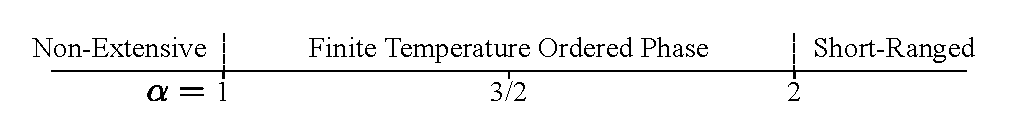
\includegraphics[width=1\textwidth,height=\textheight]{figure_code/background_chapter/alpha_diagram}
\caption[{Long Range Ising Model Behaviour}]{The thermodynamic behaviour of the long range Ising model \(H_{\mathrm{LRI}} = J \sum_{i\neq j} |i - j|^{-\alpha} S_i S_j\) as the exponent of the interaction \(\alpha\) is varied.}
\label{fig:alpha_diagram}
\end{figure}
}

\begin{Shaded}
\begin{Highlighting}[]

\end{Highlighting}
\end{Shaded}
